% *** Authors should verify (and, if needed, correct) their LaTeX system  ***
% *** with the testflow diagnostic prior to trusting their LaTeX platform ***
% *** with production work. IEEE's font choices can trigger bugs that do  ***
% *** not appear when using other class files.                            ***
% The testflow support page is at:
% http://www.michaelshell.org/tex/testflow/

\newcommand{\todo}[1]{\textbf{TODO: #1}}
\newcommand{\bas}[1]{\textbf{***BJA: #1***}}

\documentclass[conference]{IEEEtran}

\usepackage{url}
%\usepackage{breakurl}
%\usepackage[breaklinks]{hyperref}
\usepackage{graphicx}
% correct bad hyphenation here
\hyphenation{op-tical net-works semi-conduc-tor}

\begin{document}
\title{Spreadsheets are Code}

\author{\IEEEauthorblockN{Felienne Hermans, Bas Jansen, Sohon Roy, Efthimia Aivaloglou, David Hoepelman and Alaaeddin Swidan}
\IEEEauthorblockA{f.f.j.hermans, \todo{emailadresses}}
\IEEEauthorblockA{Delft University of Technology, the Netherlands}
}


\maketitle

\begin{abstract}
Spreadsheets can be considered to be the world's most successful end-user programming language. As such, many techniques from software engineering can be applied to spreadsheets. This paper details a comparison of spreadsheets to software; spreadsheets are similar in terms of applications domains, expressive power and maintainability problems. We reflect upon what makes spreadsheets successful: liveness, directness \bas{is it for every reader clear what the distinction is between liveness and directness?, For me it isn't} and an easy deployment system seems to have contributed largely to their success. In addition to success factors, we present an overview of past achievements, including spreadsheet testing, reverse engineering, smell detection, clone detection and refactoring. Furthermore, open challenges and future plans for the domain of spreadsheet professionalization are presented.
\end{abstract}

\IEEEpeerreviewmaketitle

\section{Introduction}
Spreadsheets are used for a large variety of different tasks, from invoicing to planning and from budgeting to scheduling \bas{planning, scheduling and also budgeting are a bit the same, maybe we can come up with some different examples, for example investment analysis, statistical analysis, etc.} in all sorts of domains, from small shops to multinationals. In 2004, the International Data Corporation interview \bas{interviewed} 118 business leaders and found that 85\% were using spreadsheets in financial reporting and forecasting~\cite{Panko2008}\bas{.} Especially in the financial domain, spreadsheets are ubiquitous. Financial intelligence firm CODA reported in 2008 that 95\% of all U.S. companies use spreadsheets for financial reporting~\cite{Panko2008}. The number of end-user programmers in the USA alone is conservatively estimated at 11 million \bas{And are they all excel users? is there a link between end-user programmers and excel users}, compared to only 2.75 million other, professional programmers~\cite{Scaf2005}. 

In a survey~\cite{BLS2003} held in 2003 by the US Bureau of Labor Statistics, over 60\% of 77 million surveyed workers in the US reported using spreadsheets, making this the third most common use of computers, after email and word processing. A more recent survey among 95 companies world-wide placed spreadsheets on the fourth place after email, browsing and word processing, accounting for 7.4\% of computer time~\cite{Wellnomics2007}. The Dutch Bureau of Statistics investigates computer literacy among Dutch civilians every year, and has reported a rise in people able to use formulas in a spreadsheet from 44\% to 54\% between 2006 and 2013~\cite{CBS2013}.




As artifacts of end-user programming, spreadsheets often play a role similar to source code in many companies: they support important organizational processes and sometimes \bas{I would say almost always, what could be an other reason to create a spreadsheet besides taking decisions based on the information in the spreadsheet} even business decisions are taken based on the information they contain~\cite{hermans_supporting_2011}.

While spreadsheets are commonly used, their users often have little training as programmers, but in spite of that, they often face many of the challenges of professional developers, choosing which APIs, libraries,\bas{what would be the spreadsheet equivalent of an API and / or library?} and functions to use~\cite{Ko2004}, or understanding someone else's code~\cite{Ko2011}. Since spreadsheets frequently contain errors~\cite{Panko1998}, end-users test, verify and debug their programs~\cite{Hermans2013-Cascon,Ko2004-Why}.

The above issues occurring in spreadsheets: program construction, maintenance, testing, debugging clearly occur in regular code bases too, and as such have been topics of research in the programming and software engineering community for decades~\cite{Ko2011}. Given these similarities between spreadsheets and source code, both in terms of application and issues, it is feasible to transform methods, tools and techniques from software engineering to spreadsheets, albeit sometimes in a form more tailored towards end-users. This exactly has been the approach of a number of researchers over the last decade, and this paper highlights their past achievements, challenges and future research directions. 


\section{End-user programming}
End-user programming has been a topic of study for decades, mainly started by by Nardi~\cite{Nardi1993} in her investigations into spreadsheet use in office workplaces. The difference between an end-user programmer and a professional programmer lies in their goals. It is the responsibility of a professional developer to build, debug, maintain and sometimes test software for others to use, while end-user developers create programs to support their own domain of expertise, like teaching, planning or bookkeeping~\cite{Ko2011}. As such, programs that end-users create are, by definition, not meant for others to use, while professional programming has the goal of producing code for others to use. 

The problematic aspects of end-user programming is that sometimes the created artifacts change from being a personal solution to a program used by many colleagues. When that happens, an end-user suddenly, often unintended and unprepared, has to take on challenges of professional developers, like testing, maintaining and generalizing their creations. \bas{And furthermore also when they use the spreadsheets for themselves, the software engineeering like problems do not go away. A spreadsheet for personal use suffers from the same problems that can have significant impact.}

\section{Spreadsheets are Code}
While end-user programming can take on many forms, and their users can be as diverse as system administrators~\cite{Barrett2004}, interaction designers~\cite{Ko2004, brandt_opportunistic_2008, myers_how_2008}, spreadsheets can be considered the most successful form of end-user programming. \bas{Why?} 
 % Ko also names: natural scientists [Carver et al. 2007; Segal 2007], software architects [Lakshminarayanan et al. 2006], bioinformatics professionals [Letondal 2006], web designers [Rode and Rosson 2003]


As outlined above, spreadsheets are crucial tools for many workers, enabling millions of users to do reporting, planning, scheduling and all else needed to succeed in their jobs. Obviously, not all spreadsheets are full-fledged applications: some are simply used for word processing with an easier layout and do not even contain formulas. However, spreadsheet are also commonly used to create applications, or to perform business critical calculations. We argue this second group of spreadsheets can and should be seen as source code, paving the way to apply methods from software engineering to them. In the following, we will outline three reasons that spreadsheets systems are programming languages, and spreadsheet are code.

\subsection{Application domains are similar}
Firstly, spreadsheets are used for very similar problems, like financial calculations or data manipulation. In many cases, users have investigated the use of ‘off the shelf’ solution, however, they are often expensive and do not fit their needs exactly. A second alternative, having software made specifically for their problem tends to go over time and over budget as well. In that light, using a spreadsheets seems a cheap and simple solution for many end-users.

\subsection{Expressive power is similar}

\begin{figure}
  \begin{center}
  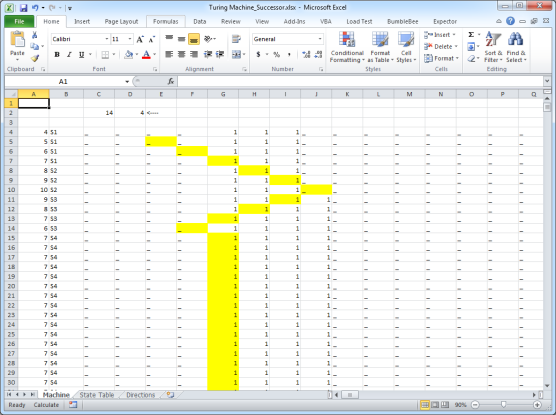
\includegraphics[width=\columnwidth]{fig/turing.png}
  \caption{A Turing machine implementation in Excel, using only formulas}
  \label{fig:visical}
  \end{center}
\end{figure} 

Secondly, spreadsheets are Turing complete, even when not take the Visual Basic for Applications code into account. Using formulas only, you can construct a Turing machine, see Figure \ref{fig:visical}~\cite{Turing2013}. 

\subsection{Maintainability issues are similar}

Finally spreadsheets suffer from typical software problems, including, but not limited to the issues below.

\textbf{Long life span} Sometimes, spreadsheets are created for one time use, and they are also thrown away after that use. More often they stay ‘alive’: enhanced with more data, reused for next year's budget or modified for a different department. Our research shows that spreadsheets have an average lifespan of five years~\cite{hermans_supporting_2011}.

\textbf{Many different users} During their lifespan, spreadsheets are frequently shared among coworkers. On average, twelve different people work with one spreadsheet during its life, in many different ways~\cite{hermans_supporting_2011}. Shared for data entry, for checking or for analysis.

\textbf{Lack of documentation} We found that only one in three spreadsheets  contain documentation, and we are not even talking about technical documentation, but just something as basic as a manual on how to use the spreadsheet is lacking in two thirds of the spreadsheets we examined.

\textbf{Quality issues} Many accounts of big impact errors: From somewhat silly errors, like an overbooked Olympic stadium~\cite{Kelso2012}, to career wrecking data analysis mistakes~\cite{Herndon2014}, the stories of errors are numerous. The European Risk Interest Group keeps a list of these ‘spreadsheet horror stories’ on their website\footnote{\url{www.eusprig.org/horror-stories}}

\section{Reflections on Spreadsheet Success factors}
Given the extreme wide adoption of spreadsheets, one could wonder why spreadsheets are as successful as they are. We believe there are a number of different reasons for their success.

\subsection{Live programming avant la lettre}

\begin{figure}
  \begin{center}
  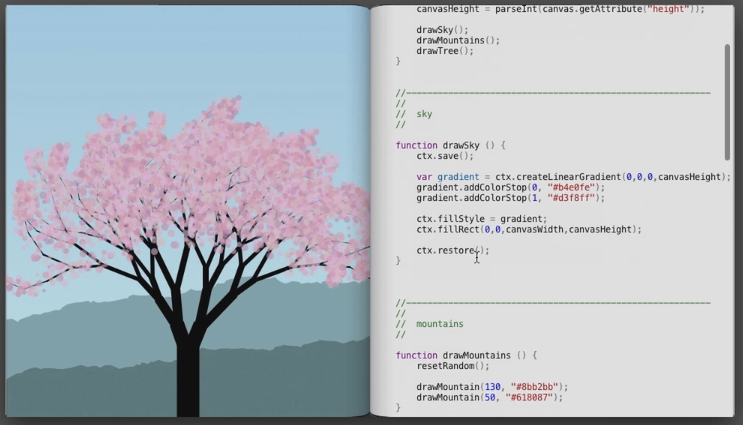
\includegraphics[width=\columnwidth]{fig/bret.png}
  \caption{Live programming: on the right the source code and on the left its instantiation of the code which changes immediately when the code is updated.}
  \label{fig:bret}
  \end{center}
\end{figure} 

Recently, ‘live programming’ has been made popular, among others by Bret Victor in his talk `Inventing on Principle'~\cite{Victor2012}. Figure \ref{fig:bret}, taken from Victor's talk, illustrates the idea of live programming: on the right, we have source code and on the right \bas{left}, we have the result of that code, in this case: a tree. Modifying the code will immediately affect the tree.
 
This idea however, often presented as a novelty in programming experiences, is exactly what happens when a user enters formulas in a spreadsheet. Immediately when the user presses enter on the keyboard, she sees the result. No compilation is needed. This liveness powers the flexibility of spreadsheets, often praised as their key success factor.

\subsection{Data, metadata and calculations in one view}
While researching spreadsheets, we have often asked the more tech savvy spreadsheet users why they did not use a more structured approach, like Microsoft Access \bas{If we are precise than Microsoft Access is a database, not a structured approach, the structured approach is not depending on the software, however using database software will force a structured approach while excel is not} . What we found was that the disconnect between the meta-data (designing the tables), the data (filling them) and the analysis (queries) was too hard for many users. The fact that all of those can be bundled in one view apparently makes it easier for non-programmers to keep an overview of what is going on. This is not that surprising, understanding dependencies of code is one of the challenges that developers still face, even advanced IDE's like Eclipse or Visual Studio do not solve this entirely. \todo{do we have a citation here?}

\subsection{One-click deployment}
Another problem that professional users face is the problem of deployment. Some more advanced users write, for example, Python scripts to analyze data. But how to get that to run on your neighbor's workstation, with a slightly different version of the operating system, a newer Office and different language settings? Spreadsheets are so universal that almost everyone has a spreadsheet program on their machine and the different programs can easily convert them. With that, a spreadsheet becomes an executable package with data and calculations packed together, that can run anywhere.\bas{nice!}

\section{Achievements} 
One of the approaches to \emph{end-user software engineering} research has been to transfer methods from software engineering to end-user languages, and this is an approach that has been applied eagerly in research into spreadsheets.  This section presents an overview of successful approaches following this scheme.

\subsection{Testing}
One of the programming concepts that found its way to spreadsheets earliest is testing. 

\todo{summarize WYSIWYT}

The WYSIWYT framework was was created~\cite{Rothermel1997} and subsequently validated~\cite{Rothermel2000} by Rothermel \emph{et al.}. Their evaluation showed that their approach had an average fault detection percentage of 81\% which is ``comparable  to  those  achieved  by  analogous  techniques  for testing  imperative  programs." Other studies have confirmed the applicability of testing~\cite{Kruck2006}. The WYSIWYT methodology requires users to explicitly indicate what cells of a spreadsheet are correct and the system propagates the testedness of a cell to its dependents. Related is the elegant work of Burnett on spreadsheet assertions that uses a similar propagation system \cite{Burnett2003}.\bas{ Shouldn't you mention Expector?}

\subsection{Reverse Engineering} 
Like software, spreadsheets often suffer from a lack of documentation. In a field study, we found that only one in three spreadsheets have documentation~\cite{hermans_supporting_2011}. This seems to be a problem especially in situation where a spreadsheet was transferred: between colleagues, from a spreadsheet user to IT for migration or when a spreadsheet had to be reviewed by an auditor. To address the lack of documentation, we developed approaches to reverse engineers spreadsheets.

\subsubsection{Extracting class diagrams}
In this approach we extracted class diagrams from spreadsheets autimatically~\cite{hermans_automatically_2010}. Spreadsheets contain groups of data, computations over these groups, and dependencies between them. This type of organization closely resembles that of object oriented systems, and thus groups of data were converted into classes, formulas into methods, and dependencies into associations. To achieve this conversion, we created a library of commonly used and well-defined spreadsheet patterns. We implemented the approach in a tool named \textit{Gyro}. The implementation was evaluated on the EUSES corpus~\cite{fisher_euses_2005}. The patterns of the created library were found to be occurring in around 40\% of the corpus spreadsheets. For 50 randomly selected spreadsheets from the corpus, class diagrams were generated manually and compared with the output of the Gyro tool. In this also, 40\% of cases proved to be exact match and the rest had various degrees of mismatch with only 12\% being totally useless.

\subsubsection{Dataflow visualization}
We did a study at a large Dutch financial services company \textit{Robeco} to ascertain the types of information needs of industrial spreadsheet users\cite{hermans_supporting_2011}. The results indicate that most important information needs of spreadsheet users concern the structure of formula dependencies. To meet this demand we conceived an approach for automatic generation of levelled data-flow diagrams from spreadsheets. The diagrams can be used to visualize data, processes that manipulate data, and the dependencies between them. Furthermore the diagrams can depict hierarchical structures like blocks of cells or different worksheets. We implemented the approach in a tool named \textit{GyroSAT}. It was evaluated with a group of 27 users from Robeco in the context of three transfer scenarios where spreadsheets were being transferred between users, from users to auditors, and from users to IT engineers who were migrating spreadsheets to custom software applications. The results indicate that the professionals from Robeco consider the tool helpful; the visualizations help them to create story lines for explaining spreadsheets to colleagues, and the visualizations scale well to large and complex spreadsheets in use at Robeco.

\subsection{Smell Detection} 
After focusing on extraction of documentation, we found out that spreadsheet users often prefer to work in spreadsheets over migrating them, hence we shifted our focus to helping users understand the complexity of spreadsheets and determine ways to improve them. For this, we took the idea of \emph{code smells} as inspiration, adapting it however, to be applicable to spreadsheets. \todo{hier ook het ICSE paper van SC and Cunha}

\subsubsection{Formula-level Smell detection}
We started by defining smells on the formula level where we found that many smell defined for code also applied nicely to spreadsheets~\cite{hermans_detecting_2014}. As an example, consider conditional complexity. Since spreadsheets support conditionals too, spreadsheet formulas too \bas{2x too} can suffer from conditional complexity, when many IFs are nested within one formulas. Other code smells need small modifications to be applicable to spreadsheets: the `many parameters' smell became `many references': a formula that references a long list of different ranges in a spreadsheet is as smelly as a method with lots of parameters. After defining the smells for spreadsheets, we performed empirical evaluations for ascertain ourselves the smells mattered to spreadsheet users. We first analyzed the occurrence of the smells with the EUSES corpus~\cite{fisher_euses_2005}, secondly, we conducted a series of case studies at Robeco, where we conducted ten case studies. 

In more recent work we have compared two datasets: one of which users expressed that they were unmaintainable, and a version of the same spreadsheet improved, one could say refactored, by professional spreadsheet developers. The results shows that the improved versions suffered from smells to a lesser degree, increasing our confidence that presence of smell indeed coincides with users finding spreadsheets hard to maintain~\cite{Jansen2015}.

\subsubsection{Structural Smell detection}
In addition to smells within a single worksheet of a spreadsheet, smells can occur in the way they are coupled also; just like with source code. We explored this phenomena too, leading to four `inter-worksheet smells': Inappropriate Intimacy, Feature Envy, Middle Man and Shotgun Surgery~\cite{hermans_detecting_2012-1}. We again performed a quantitative and qualitative evaluation of our approach. Firstly, we analyzed the EUSES~\cite{fisher_euses_2005} corpus, and investigated the occurrence of inter-worksheet smells. Secondly, we conducted a series of case studies at the above described company Robeco, where we conducted ten case studies. In each study we analyzed a real-life spreadsheet, and discussed the located smells with the spreadsheet owner. \bas{and what were the results / conclusions / contributions of this study?} 

\subsection{Clone detection}
Finally, we also investigated the occurrence of clones within spreadsheets, or `copy-pasting'~\cite{hermans_data_2013}. While copy-pasting in spreadsheets is common: spreadsheet users mimic abstraction by copying a similar formula down or left over multiple rows or columns, some forms of copying are error prone. In our research we have focused on \emph{data clones}: copies made with the `paste as values' option within Excel. We have designed a detection algorithm to help spreadsheet users in finding errors and improving the quality of their calculations, based in existing clone detection algorithms working on source code~\cite{DBLP:conf/cascon/Johnson93}. In addition to exact clones, we can also detect \emph{near-miss clones}, those where minor to extensive modifications have been made to the copied fragments\cite{DBLP:conf/icsm/Roy09}.

Our approach was subsequently validated both quantitatively and qualitatively. Firstly, we analyze the EUSES corpus~\cite{fisher_euses_2005} to calculate the precision and performance of our algorithm and to understand how often clones occur. 
Secondly, we perform two case studies: one with a large budget spreadsheet from our own university and a second one for a large Dutch non-profit organization, for which we analyzed 31 business critical spreadsheets.

Recently, there have been other efforts to apply clone detection to artifacts other than source code, Alalfi \emph{et al.}~\cite{DBLP:conf/icsm/Alalfi2012} have successfully applied clone detection to Simulink models. For this purpose they adapted NiCad and were able to efficiently find exact, renamed and near-miss clones in Simulink models.
\bas{to what extend is this relevant for clone detection in spreadsheets?}

\subsection{Improving/re-engineering/Refactoring}
A final direction on which end-user research has focused is---a logical step after research on smells---is refactoring of end-users artifacts. 

%The first attempt to define refactorings for spreadsheets was made by O'Beirne, who took inspiration from both existing source code refactorings and his own experience in working with spreadsheets, he however did not evaluate his approach~\cite{obeirne_spreadsheet_2010}. 

Inspired by our work on spreadsheet smells, Badame and Digg~\cite{badame_refactoring_2012} developed a tool called RefBook that supported a number of refactorings for spreadsheet formulas including extract column, replace awkward formula, string to dropdown, introduce cell name, and extract literal. While some of their refactorings can relieve known code smells---for example extract column makes formulas shorter, thus addressing multiple operations---their refactorings were not directly related to smells. RefBook was evaluated on 28 users in an online experiment showing that RefBook increases spreadsheet programmer
productivity, increases the reliability of transformations, and increases the quality of spreadsheets. Furthermore they studied the EUSES corpus to show that their refactorings can be widely applied. For example, in 27\% contain some form of duplication, so Extract Column could be applied to simplify the spreadsheet.

We subsequently defined refactorings corresponding to our smells~\cite{hermans_detecting_2014} and applied them to the 10 spreadsheets received from financial company Robeco, demonstrating a combination of one or more refactorings from our set could relieve smells in 87\% of smelly formulas.

\subsection{Conclusion}
In conclusion, we can state that many approaches useful for source code are applicable to end-user programming in general and spreadsheets in particular, from testing to smells and from refactoring to reverse engineering, end-users benefit from it as much as professional developers do.

%This all has to do with understanding and improving quality we still want to support understanding domain/calculation.Our work and that of others was all 100\% automated, what we have learned, if we want to continue with reverse engineering, we need more support from the user, both the creator and human level intelligence (a generic user): we both want to do large studies with generic users like the labeling game and make support for users to add more (domain) knowledge to the sheets.

\section{Challenges} 
Now we have described the key success in the application of software engineering to spreadsheets, we direct our attention to challenges that still lie ahead of us. 

\subsection{End-user's perception and self perception}
One of the core challenges of performing research on end-user programming in general, is that users do not seen themselves as programmers.  In one case where we were working with an investment banker, who was even insulted when we, impressed with a risk management dashboard he built with Excel, called him a programmer. Because end-user programmers do not self identify as developers, they often are not aware of tools, methods and techniques that could support them in their programming efforts.

The perception of end-user programmers as not being `real' programmers is not limited to how programmers view themselves, but also to how they are seen by others. Coworkers, especially those themselves trained as professional developers, often fail to recognize and sometimes even belittle their programming efforts, while professional developers in the workplace could offer great support and could ease our technology transfer issues. \bas{especially in the 'structured' translation of domain specific knowledge to technical implementation}

\subsection{Lack of Best Practices}
A challenge that follows the previous one is the lack of standards. As spreadsheets and their creators are not seen as source code and programmers respectively, they are often outside of the scope of a diverse range of professionalization efforts within companies. Software, but also numerous processes are standardized; spreadsheets on the other hand are rarely. While a number of spreadsheet standards exist\footnote{\url{http://www.fast-standard.org/}}\footnote{\url{http://www.ssrb.org/standards}}\footnote{\url{http://www.spreadsheetsafe.com/}}, these have to date not found widespread adoption, nor are there lint tools \bas{lint tools?} for spreadsheet compliance available. 

The lack of standards means spreadsheets can be made in many different ways, this in turn inhibits easy comprehension and maintenance, but also makes it harder to automatically analyze and process of \bas{delete of} spreadsheets.

\subsection{Lack of Data}
Spreadsheets often contain models and calculations of vital information to companies and therefore companies are often reluctant to share them with researchers. This is an large challenge with industrial research in general, and spreadsheets in specific. Contrary to source code, which developers often happily open source, and share on online platforms like GitHub, spreadsheet users typically do not share their applications. While there are a number of public datasets available~\cite{fisher_euses_2005, Hermans2015, conf/msr/BarikLSSM15}, only one of these(\cite{Hermans2015}) stems from a company. And even then, we lack information about their creation and maintenance process process around them. Information that is often available for source code repositories, like issues, refactorings and version control history, are missing from spreadsheets, prohibiting us from deeply understanding the problems with spreadsheets. We have worked together with companies providing us with data~\cite{hermans_supporting_2011, hermans_detecting_2012, hermans_detecting_2012-1, hermans_detecting_2014, Jansen2015} enabling us to study spreadsheets \emph{in the wild}, however unfortunately, that came at the price of reduced repeatability, as we were not allowed to share these spreadsheets.

\subsection{Size of spreadsheets}
While many spreadsheets are relatively small, spreadsheets can also grow extremely large over their long lifespan. The biggest spreadsheet form the Enron set had no less than 175 worksheets, and about 10\% of spreadsheets in the corpus have 10 or more worksheets. Large spreadsheets, especially those with heavy connections between the worksheets, make it hard for users to  understand and maintain it. There have been several efforts to support spreadsheets users in comprehension \todo{Sohon maybe you can add some work from your SEMS paper?} but while these tools typically perform well on toy examples, industrial adoption seems to be far away for real-life spreadsheets, as 1) tools get unreasonably slow on large spreadsheets and 2) the abstractions in the visualization quickly lose their power for large spreadsheets with loads of dependencies. \todo{Sohon do you have a nice example?}

%For useful visualization we have to leave the cell level, want to look at the computation level (slicing)

\subsection{Performance}
Understandability and maintainability are not the only issues with large spreadsheets, large spreadsheets can have from serious performance problems too. We have seen in practice that especially spreadsheets using Monte Carlo simulations often suffer from performance problems. Some solutions have been proposed for this \todo{Alaaeddin, can I steal your related work here?}

\subsection{Technical issues} \bas{tekst loopt niet lekker, what is the link with SCAM HPC/HEAT, more explanation about undo/redo stack, etc.}
Finally, there are technical issues in processing spreadsheets and developing add-ins for a proprietary product like Microsoft Excel. 
Lack of open standards, and even when open, not very standardized (we have to reverse engineer stuff, link SCAM, also HPC/HEAT is not open, not willing to share)
Limited options for customization (undo/redo stack is not available, in the object model precedents do not go deeper than 1 level, objects model gets extended but not updated)

Obviously, one could steer away from these issues by implementing a system themselves (Forms/3 and Sestoft) or to build plugins for open source tools. Here however the tradeoff with realism is apparent too, building tools for Excel which is the number 1 spreadsheet solution increase the realism and impact of research tools.

\section{Future opportunities}
Given the above achievements  and challenges, we identify the following viable directions for future work in the area of spreadsheet software engineering.

\subsection{Continuation of the refactoring and testing work}
In contrast to the work on smells that have been tried in practice and spurred numerous follow up works and has been picked up by a larger research community, refactorings and testing need to be made more applicable.

\subsection{More deeply understanding the role of spreadsheets in the enterprise}
This understanding will have to happen both culturally (evolution, process) and in their application (use of spreadsheets) For example, classification different types of spreadsheets, potentially. For this we are exploring the following concrete endeavours:

\subsubsection{For the purpose of reverse engineering (Sohon)}
Potential application of extraction high level structure would be:
\paragraph{documentation extraction}
\paragraph{validating spreadsheets at a higher level}

\subsubsection{To support users in creating better spreadsheets}
Using  an alternative interface for some types of spreadsheets, bringing a higher level of abstraction (Bas)

\subsection{Beyond formulas}

  Self-service BI. This field is now mainly concerned with building but not with maintenance. We see them making the same mistake by not focusing on end-user maintenance, maybe underestimating the longevity of the new artifacts created. We suspect that this new incarnation of end-user programming again will suffer from smells etc. So our research will explore this, for example by focusing. Other spreadsheet concepts like PivotTables and VBA code
  

Increasing performance of spreadsheets (Allaeddin)
Intertwining of formulas and other constructs makes automated analysis even harder



\section{Conclusion}
This paper presents an overview of research papers on applying methods from software engineering to spreadsheets. We first makes the case that spreadsheets are code: they are used for similar problems, have similar expressive power and suffer for similar problems. We then reflect upon the success of spreadsheets, what makes them the world's most used programming languages for end-users? We assert their liveness, directness and easy deployment are core contributors to their widespread adoption. \bas{achieved research, challenges and future opportunities are missing}






% trigger a \newpage just before the given reference
% number - used to balance the columns on the last page
% adjust value as needed - may need to be readjusted if
% the document is modified later
%\IEEEtriggeratref{8}
% The "triggered" command can be changed if desired:
%\IEEEtriggercmd{\enlargethispage{-5in}}


\bibliographystyle{IEEEtran}
% argument is your BibTeX string definitions and bibliography database(s)
\bibliography{references}


% that's all folks
\end{document}


